\chapter{Conclusão}
\label{chap4}

\begin{figure}[H]
\centering
\color{red}
\setlength{\abovecaptionskip}{-20pt}
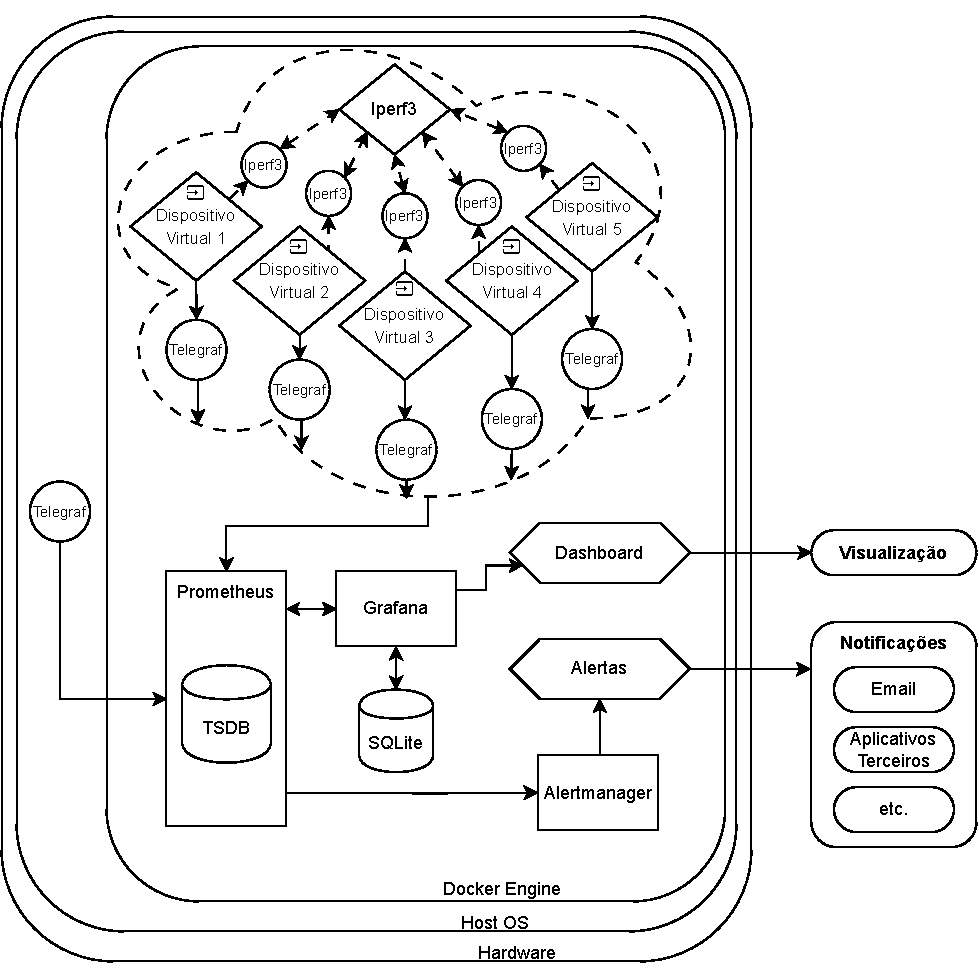
\includegraphics[width=\textwidth]{Imagens/chap04/final_diagram.pdf}
\caption{Arquitetura final.}
\label{fig:DiagramaFinal}
\end{figure}

\begin{figure}[H]
\centering
\color{red}
\setlength{\abovecaptionskip}{-20pt}
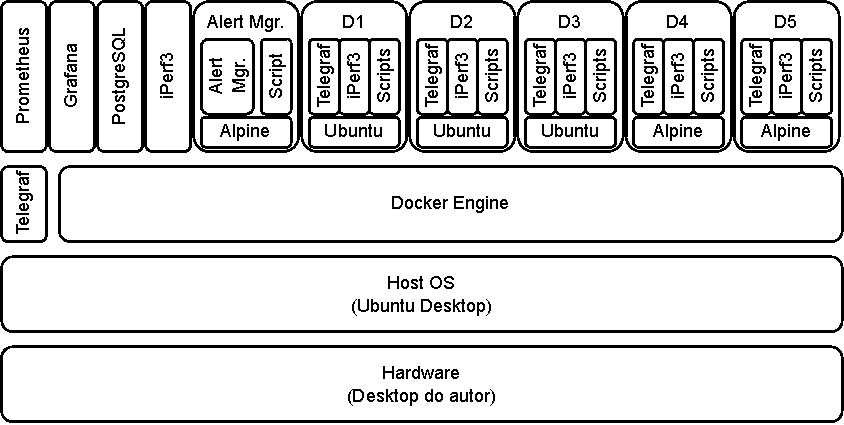
\includegraphics[width=\textwidth]{Imagens/chap04/final_stack.pdf}
\caption{\foreign{Stack} final.}
\label{fig:StackFinal}
\end{figure}

%comentar as discussoes para validação comparativa, que eventualmente foi desconsidarada por nao ter equipamento


% Mas fica a reflexão: faz sentido comparar métricas entre dispositivos virtuais? Quando o objetivo era comparar máquinas físicas versus containers, essa comparação qualitativa era justificável. Porém, ao comparar container versus container, será que essa análise ainda se sustenta? Há valor prático em comparar dispositivos virtuais entre si nesses termos?

% --> Realmente não faz sentido, logo não é necessário fazer esse levantamento.

%TODO: Em trabalhos futuros a análise de viabilidade de implementação em NUC ou Raspberry Pi
